%Stanford, August 14, 2016
\documentclass[10pt,compress,xcolor={usenames,dvipsnames}]{beamer} %slides and notes
\usepackage{amsmath,datetime,xmpmulti,mathtools,bbm,array,booktabs,alltt,xspace,mathabx,pifont,tikz,calc,colortbl,graphicx}
\usepackage[usenames]{xcolor}
\usepackage[tikz]{mdframed}
\usepackage[author-year]{amsrefs}
\usepackage{newpxtext}
%\usepackage{newtxtext}
%\usepackage{newtxmath}
\usepackage[euler-digits,euler-hat-accent]{eulervm}
\usetikzlibrary{arrows}
\usepackage{cleveref}
\usetheme{FJHSlimNoFoot}

\definecolor{ltred}{rgb}{1,0.75,0.75}

\setlength{\parskip}{2ex}
\setlength{\arraycolsep}{0.5ex}


\mdfdefinestyle{redshade}{%
	leftmargin=0 pt,
	rightmargin = 0pt,
	innerleftmargin = 1ex,
	innerrightmargin = 1ex,
	skipabove = 0 pt,
	skipbelow = 0 pt,
	backgroundcolor=red!20,
	linecolor=red!20,
	roundcorner=5pt}

\title[]{Error Analysis of (Quasi-)Monte Carlo Methods}
\author[]{Fred J. Hickernell}
\institute{\small{Department of Applied Mathematics,  Illinois Institute of Technology \\
\href{mailto:hickernell@iit.edu}{\url{hickernell@iit.edu}} \quad
\href{http://mypages.iit.edu/~hickernell}{\url{mypages.iit.edu/~hickernell}} 
\\[2ex]
Joint work with Llu\'is Antoni Jim\'enez Rugama \\[2ex]
Supported by NSF-DMS-1522687}}
\date[]{August 14, 2016}

%Title:  Guaranteed Fixed-Width Confidence Intervals for Monte Carlo and Quasi-Monte Carlo Simulation

%Abstract: When performing a simulation to determine $\mu=\mathbb{E}(Y)$ one wonders what the error is and how many samples are required to achieve a desired accuracy.  We may want a confidence interval for the of the form $\mathbb{P}[\lvert\mu - \hat{\mu}_n\rvert\le \varepsilon] \ge 99\%$ where $\varepsilon$ is fixed by the user, and the number of samples, $n$, must be determined to make the sample mean, $\hat{\mu}_n$ close enough to the true mean.  Popular confidence intervals are based on large sample results, such as the Central Limit Theorem, or heuristics, but these error estimates can be fooled.  We explain how these popular estimates can fail and present new, guaranteed, fixed-width confidence intervals for  simple Monte Carlo and quasi-Monte Carlo simulation.   Moreover, we provide upper bounds on the required sample sizes  that show a reasonable dependence on the unknown difficulty of the simulation.



\input FJHDef.tex
\renewcommand{\mSigma}{\Sigma}
\newcommand{\smallcite}[1]{{\small\cite{#1}}}
\newcommand{\smallocite}[1]{{\small\ocite{#1}}}
\newcommand{\smallcites}[1]{{\small\cites{#1}}}
\newcommand{\tol}{\text{tol}}
\newcommand{\Phnu}{\Prob_{\hnu}}
\DeclareMathOperator{\oerr}{\overline{err}}
\DeclareMathOperator{\cubMC}{cubMC}
\DeclareMathOperator{\qse}{qse}
\DeclareMathOperator{\integ}{int}
\DeclareMathOperator{\trap}{trap}
\DeclareMathOperator{\size}{size}
\DeclareMathOperator{\app}{id}
\DeclareMathOperator{\err}{err}
\DeclareMathOperator{\MSE}{MSE}
\DeclareMathOperator{\RMSE}{RMSE}
\DeclareMathOperator{\PProb}{\mathbb{P}}
\DeclareMathOperator{\walsh}{walsh}
\newcommand{\happ}{\widehat{\app}}
\newcommand{\hinteg}{\widehat{\integ}}
\newcommand{\cube}{[0,1)^d}
\newcommand{\desall}{\{\vz_i\}}
\newcommand{\desn}{\{\vz_i\}_{i=0}^{n-1}}
\def\newblock{\hskip .11em plus .33em minus .07em}
\newcommand{\wcS}{\widecheck{S}}
\newcommand{\wcomega}{\widecheck{\omega}}
\newcommand{\HickernellFJ}{H.} %To give my name to the bibliography
\newcommand{\abstol}{\varepsilon_{\text{a}}}
\newcommand{\reltol}{\varepsilon_{\text{r}}}
\DeclareMathOperator{\algn}{ALN}
\DeclareMathOperator{\disc}{DSC}
\DeclareMathOperator{\Var}{VAR}
\DeclareMathOperator{\GP}{\cg\cp}
\newcommand{\Dt}{\text{D}}
\newcommand{\Rn}{\text{R}}
\newcommand{\Ba}{\text{B}}
\newcommand{\tmC}{\widetilde{\mC}}
\newcommand{\tvC}{\widetilde{\vC}}
\newcommand{\vC}{\boldsymbol{C}}

\newcommand{\redroundmathbox}[1]{\parbox{\widthof{$#1$\hspace{1em}}}
	{\begin{mdframed}[style=redshade]\centering $#1$ \end{mdframed}}}

\newcommand{\medcone}{\parbox{1.2cm}{\includegraphics[width=0.55cm,angle=270]{ProgramsImages/MediumWaffleCone.eps}}\xspace}

\newcommand{\smallcone}{\parbox{0.65cm}{\includegraphics[width=0.3cm,angle=270]{ProgramsImages/MediumWaffleCone.eps}}\xspace}

\newcommand{\lecone}{\smallcone\hspace*{-0.3cm}\mathclap{\le}\hspace*{0.35cm}}

\definecolor{MATLABBlue}{rgb}{0, 0.447, 0.741}
\definecolor{MATLABOrange}{rgb}{0.85,  0.325, 0.098}
\definecolor{MATLABPurple}{rgb}{0.494,  0.184, 0.556}
\definecolor{MATLABGreen}{rgb}{0.466,  0.674, 0.188}



\begin{document}
\tikzstyle{every picture}+=[remember picture]
\everymath{\displaystyle}

\frame{\titlepage}

\section{Examples}
\begin{frame}
	\frametitle{Integration Examples}
	\vspace{-8ex}
	\begin{tabular}{m{8cm}m{3cm}}
	\[ \begin{aligned}
	\mu &= \frac{1}{N} \sum_{j=1}^N f(j) = \text{population average hours of sleep} \\ f(j) & = \text{hours of sleep for individual } j 
	\end{aligned} \]
	& \href{http://www.preapps.com/blog/wp-content/uploads/2015/09/Valuable-Sleep.jpg}{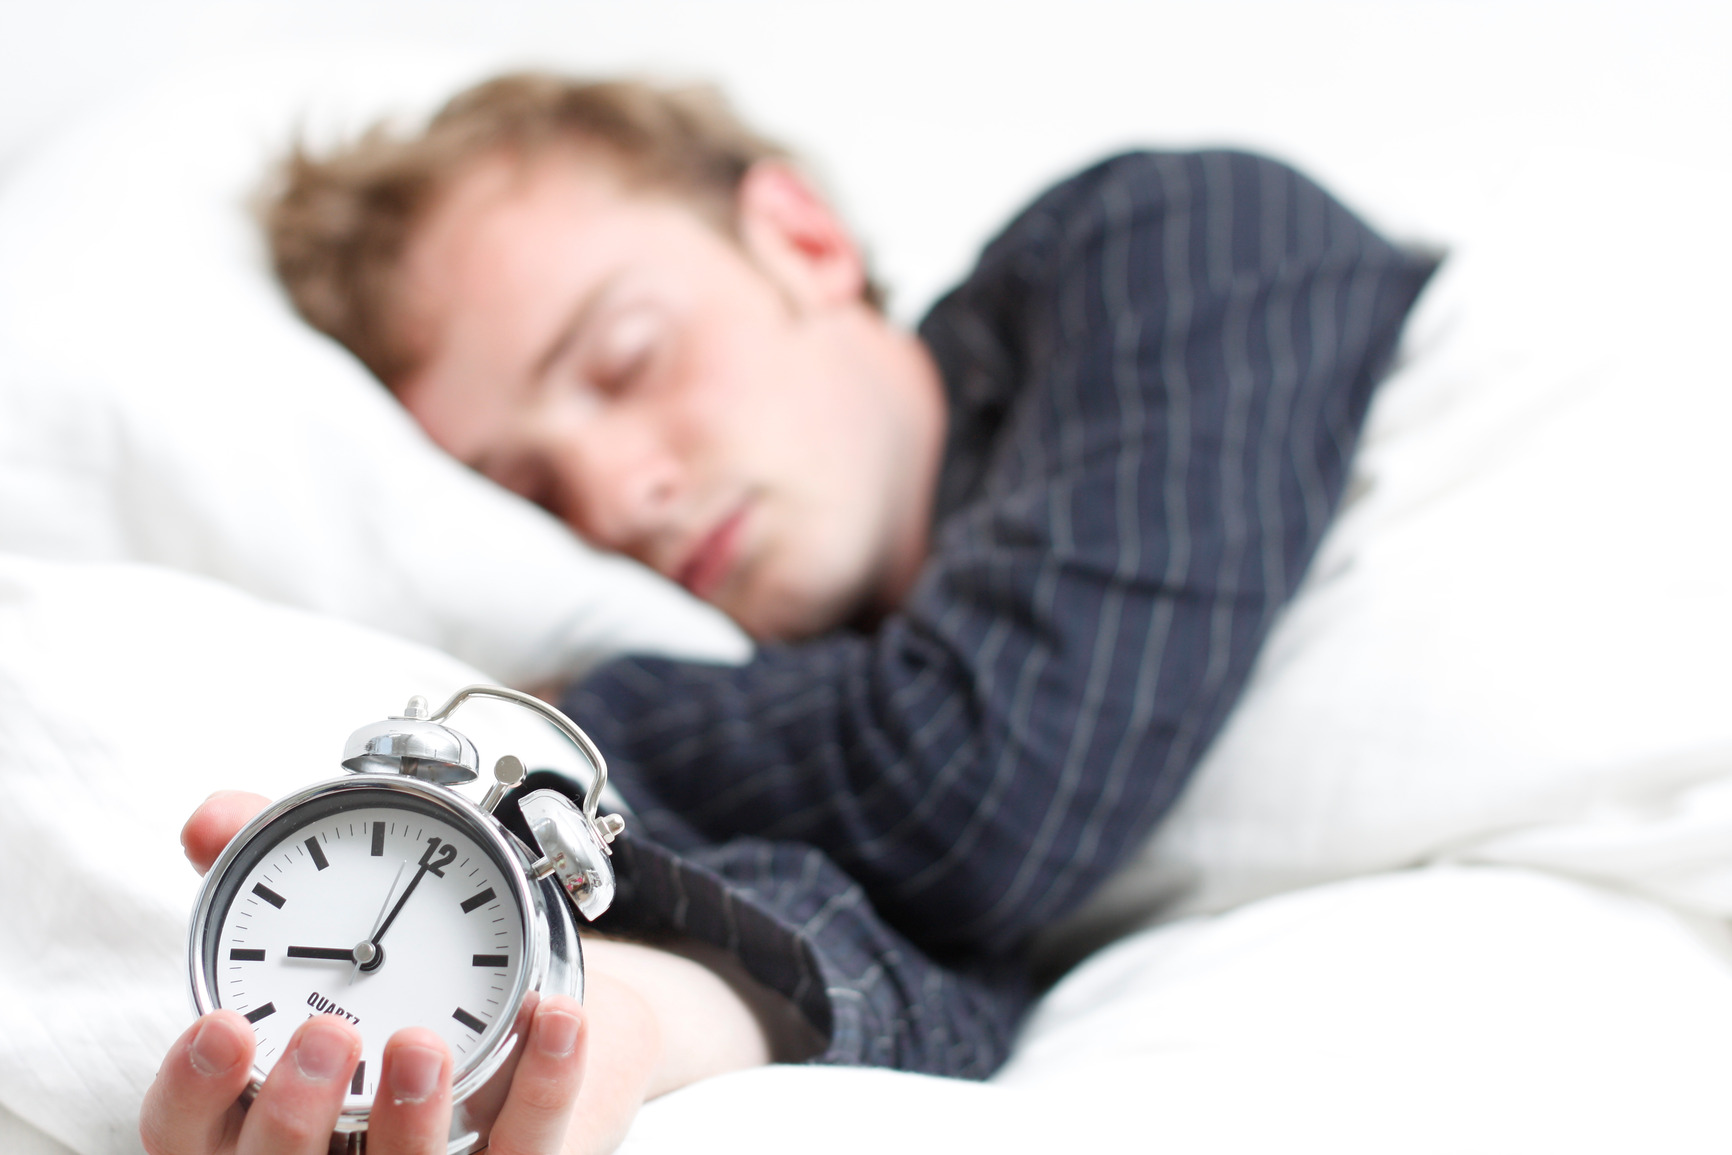
\includegraphics[width = 3cm]{ProgramsImages/Valuable-Sleep.jpg}}
\uncover<2->{
	\tabularnewline [-2.2ex] \arrayrulecolor{ltred}\toprule
\tabularnewline [-2.6ex] 
\vspace{-4ex}
		\[ \begin{aligned} \mu &= \int_{\reals^d} f(\vx) \, \nu (\dif \vx) =  \text{option price}\\ f(\vx) & = \text{discounted payoff determined by innovations }\vx
			\end{aligned} \] 
		& \href{http://i2.cdn.turner.com/money/dam/assets/130611131918-chicago-board-options-exchange-1024x576.jpg}{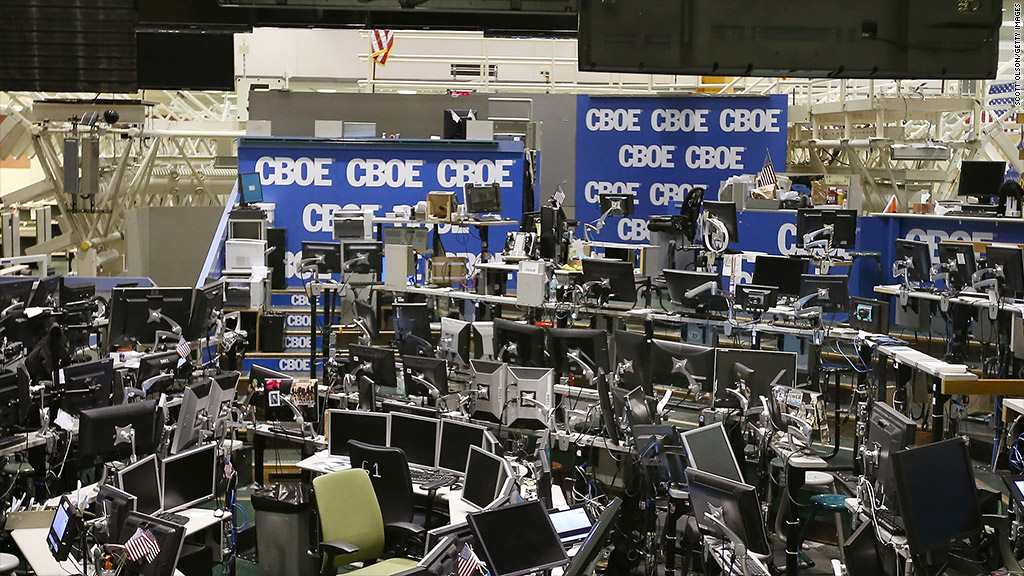
\includegraphics[width = 3cm]{ProgramsImages/130611131918-chicago-board-options-exchange-1024x576.jpg}}
		} 
	 \uncover<3->{
	 	\tabularnewline [-2.2ex] \arrayrulecolor{ltred}\toprule
\tabularnewline [-3.6ex] 
\vspace{-3ex}
	 	\[ \begin{aligned}\mu &= \int_{\cx} g(\vx) \, \dif \vx = \Prob(\vX \in \cx) = \text{probability} \\ g & = \text{probability density function}
	 		\end{aligned} \] 
	 		& \href{http://www.mathworks.com/matlabcentral/answers/uploaded_files/26298/Plotting\%20a\%203d\%20gaussian\%20function\%20using\%20surf\%20-\%202015\%2002\%2027.png}{\includegraphics[width = 3cm]{ProgramsImages/Plotting_gaussian.png}}
	 		} 
	 \uncover<4->{
	 	\tabularnewline [-4.2ex] \arrayrulecolor{ltred}\toprule
\tabularnewline [-6ex] 
\[ \begin{aligned}
	 	\mu & = \int_{\cx} f(\vx) \, \nu(\dif\vx) \uncover<5->{\approx \hmu = \sum_{i=1}^n f(\vx_i) w_i = \int_{\cx} f(\vx) \, \hnu(\dif\vx)}
	 		\end{aligned} \]
	 		& \uncover<6>{%\parbox{2ex}{\phantom{a}}\newline 
	 			%\phantom{Hicke}
	 				\qquad \redroundmathbox{\mu - \hmu =\, ?}}}
	 			\tabularnewline[-6ex]
	 	\multicolumn{2}{m{11.7cm}}{%
	 	\uncover<4->{\[ 
	 	\nu = \text{probability measure} \uncover<5->{, \quad\hnu = \sum_{i=1}^n w_i \delta_{\vx_i} = \text{sampling measure},\quad \sum_{i=1}^n w_i =1}
	 	 \] }}		
	\end{tabular}
	

\end{frame}

\section{Trio Error Identity}

\begin{frame}
	\frametitle{Trio Identity for the Error \cite{Men16a}}
	\vspace{-7ex}
	\begin{align*}
	 \redroundmathbox{\mu - \hmu} &= \int_{\cx} f(\vx) \, \nu(\dif\vx) - \sum_{i=1}^n f(\vx_i) w_i = \int_{\cx} f(\vx) \, (\nu - \hnu)(\dif\vx) \\
	& \uncover<2->{=  \redroundmathbox{\algn(f,\nu - \hnu) \, \disc(\nu - \hnu) \, \Var(f)} \\[1ex]
	\Var(f) & =  \text{\alert{variation} of the integrand from a constant} \ge 0 \\
	\disc(\nu - \hnu) & =  \text{\alert{discrepancy} of the sampling measure }\\
	 &  \qquad \qquad \qquad  \text{from the probability measure} \ge 0\\
	\algn(f,\nu - \hnu) & =  \text{\alert{alignment} of the integrand and} \\
	&  \qquad \qquad \qquad \text{the difference between the two measures}
\only<2>{\\ & \qquad \qquad \qquad \text{\alert{often ignored}}}}
	\end{align*}
	
	\only<1-3>{\uncover<3>{\vspace{-2ex}\begin{itemize}
			\item Reduce error by clever sampling, $\hnu$
			\item Reduce error by rewriting the problem while leaving $\mu$ unchanged
			\item Improve understanding of error by modifying $\disc$ and $\Var$ to reduce $\disc(\nu - \hnu) \, \Var(f)$
			\item Determine the sample size $n$ needed to make $\abs{\mu - \hmu} \le \varepsilon$
		\end{itemize}}}
		
	\only<4>{\vspace{1ex}\centerline{\begin{tabular}{r@{\quad}@{\quad}c@{\qquad}c}
		\multicolumn{1}{c}{}& \multicolumn{2}{c}{Sampling Distribution, $\hnu$}\\
		 Integrand, $f$ & Fixed & Random \\  \cmidrule[1.5pt]{2-3} \\   [-1ex]
		 Fixed & Deterministic & Randomized \\ [1ex]
		Gaussian Process	& Bayesian & Bayesian Randomized	
	\end{tabular}}}

\end{frame}

\begin{frame}
	\frametitle{Deterministic Trio Identity}
	\vspace{-8ex}
	\begin{align*}
	(\cf, \norm[\cf]{\cdot}) & = \text{normed vector space of integrands} \\
	& \qquad f \mapsto f(\vx) \text{ is bounded for all } \vx \in \cx \\
	& \qquad L: \cf \to \reals \text{ is bounded and linear}, \quad 1 \in \cf \text{ or } L(f):=0  \\
	(\cm, \norm[\cm]{\cdot}) & = \text{normed vector space of signed measures, includes } \delta_{\vx} \ \forall \vx \in \cx\\
	& \qquad  \norm[\cm]{\lambda} := \sup_{\substack{f \in \cf \\ f \ne 0= L(f)}} \frac{\abs{\int_{\cx} f(\vx) \, \lambda(\dif\vx)}}{\norm[\cf]{f}} = \text{norm of } f \mapsto \int_{\cx} f(\vx) \, \lambda(\dif\vx)\\
	\uncover<2->{\redroundmathbox{\mu - \hmu} &= \int_{\cx} f(\vx) \, (\nu - \hnu)(\dif\vx) \\
	& =  \redroundmathbox{%
		\underbrace{\frac{ \int_{\cx} f(\vx) \, (\nu - \hnu)(\dif\vx)}{\norm[\cm]{\nu - \hnu} \norm[\cf]{f-L(f)}}}_{\textstyle \algn^\Dt(f,\nu - \hnu)} \, \underbrace{\norm[\cm]{\nu - \hnu}}_{\textstyle\disc^\Dt(\nu - \hnu)} \, \underbrace{\norm[\cf]{f-L(f)}}_{\textstyle\Var^\Dt(f)}}}
	\end{align*}
	\vspace{-4ex}
	\uncover<2->{\begin{itemize}
			\item $\abs{\algn^\Dt(f,\nu - \hnu)}   \le 1$  by the definitions of $\norm[\cf]{\cdot}, \norm[\cm]{\cdot}$
			\item Ignoring $\algn^\Dt(f,\nu - \hnu)$ yields a generalized Koksma-Hlawka inequality \cites{Nie92,Hic97a,Hic99a}
		\end{itemize}.}
\end{frame}

\begin{frame}
	\frametitle{Hours of Sleep Web Survey}
	\vspace{-8ex}
	\begin{tabular}{m{8cm}m{3.5cm}}
		\begin{gather*}
		\mu = \text{population average hours of sleep} \\
		f(j) = \text{hours of sleep for individual } j \\
			\nu = \frac{1}N \sum_{j=1}^N \delta_{j} = \text{uniform}, \qquad \hnu  = \frac 1n \sum_{i=1}^n \delta_{x_i}\\
			\{x_i\}_{i=1}^n \text{is a sequence of distinct individuals}, \quad n < N
			\end{gather*}
			&
	\href{http://www.preapps.com/blog/wp-content/uploads/2015/09/Valuable-Sleep.jpg}{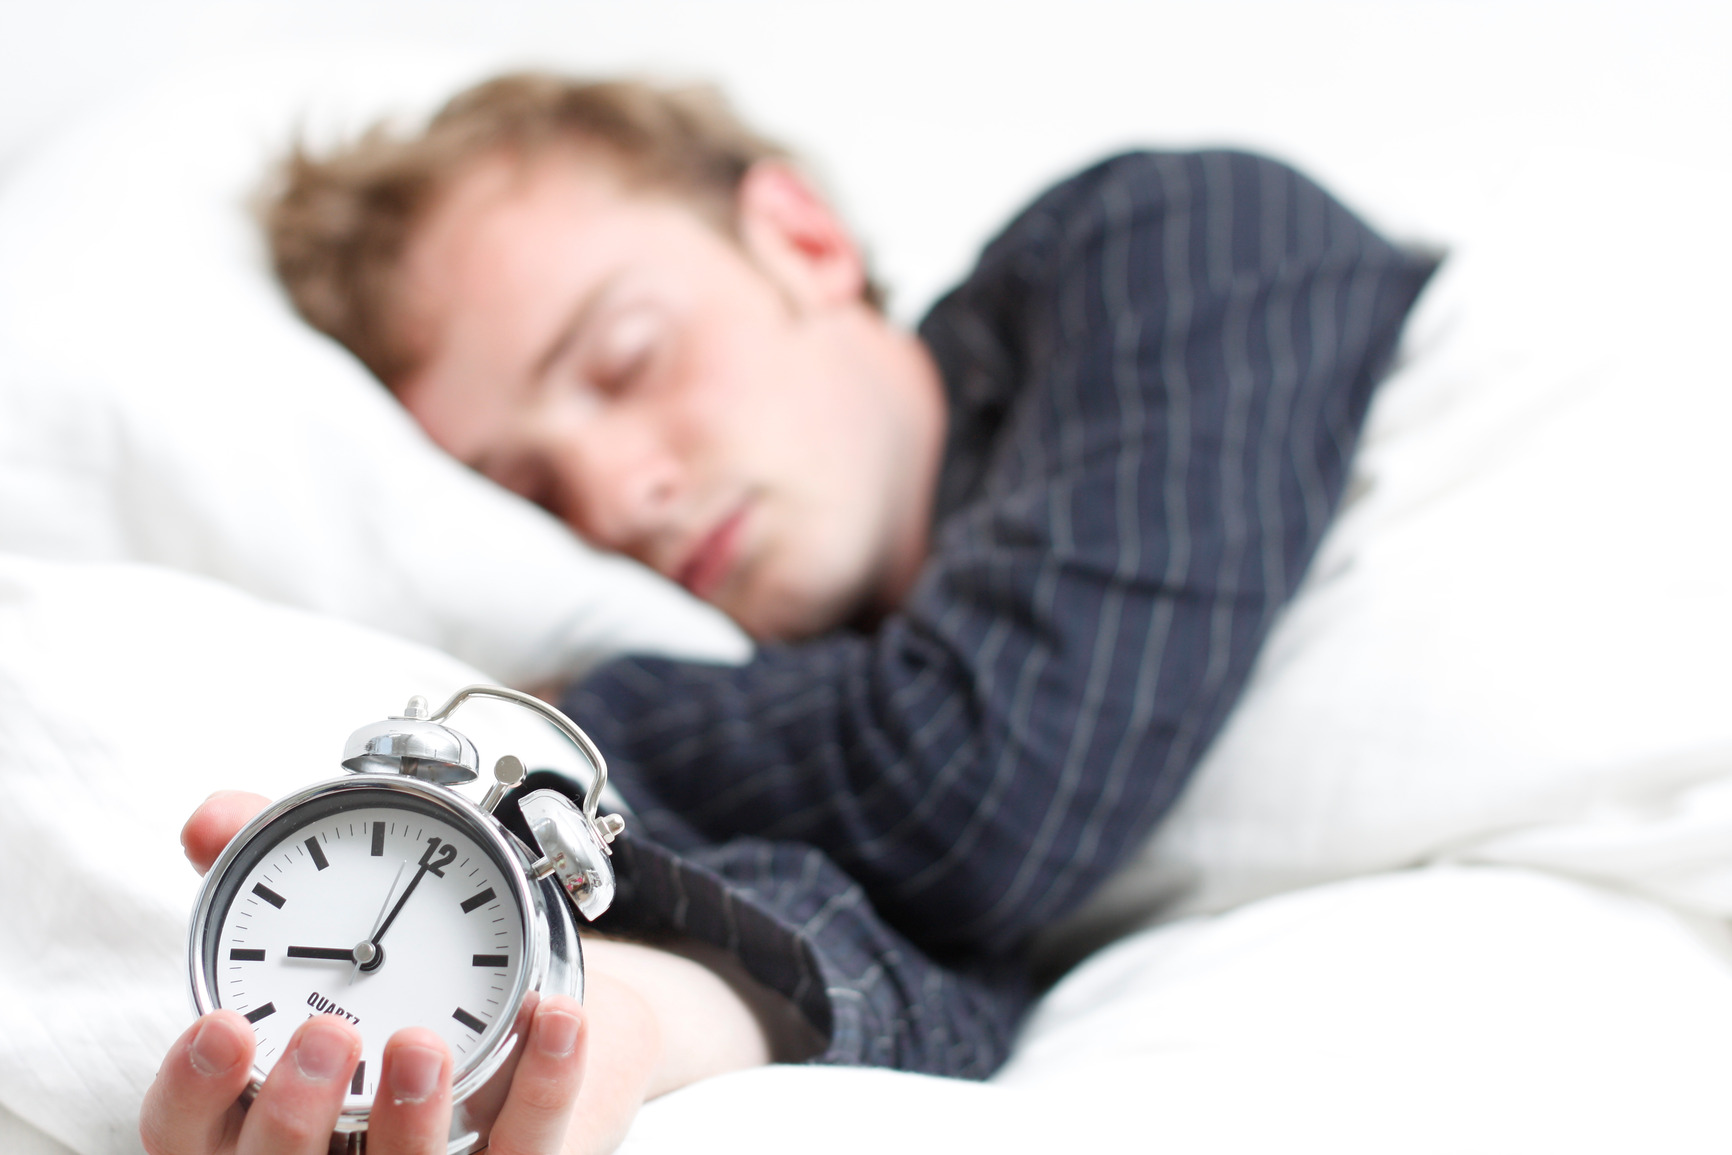
\includegraphics[width = 3cm]{ProgramsImages/Valuable-Sleep.jpg}}
	\end{tabular}
	\vspace{-4ex}
	\[L(f)  = \frac 1N \sum_{j=1}^N f(j) = \mu, \qquad \cov(f,g) = \frac 1N \sum_{i=1}^N [f(j) - L(f)][g(j) - L(g)]\]
	\centerline{\redroundmathbox{\mu - \hmu  = 
			\underbrace{-\corr\bigl(f, \bbone_{\{\vx_i\}_{i=1}^n}\bigr)}_{\textstyle\algn^\Dt(f,\nu - \hnu)}
			\underbrace{ \sqrt{\frac{1-n/N}{\alert{n/N}}}}_{\textstyle\disc^\Dt(\nu - \hnu)}
			\underbrace{ \std(f)}_{\textstyle\Var^\Dt(f)} }}
		\vspace{-2ex}
		\begin{itemize}
			\item Discrepancy depends on the \alert{sample fraction}, not merely the sample size.  
			
			\item Discrepancy may be large if the sample fraction is small
			
			\item \alert{Correlation} for a web survey is difficult to predict or control
		\end{itemize}
\end{frame}

\begin{frame}
	\frametitle{Reproducing Kernel Hilbert Spaces (RKHS)}
	\vspace{-4ex}
	If the space of integrands, $\cf$ is a Hilbert space with \alert{reproducing kernel} $K$, then the cubature error can be expressed as an inner product of the integrand with the representer for the error functional:
	\begin{align*}
	\Var(f) &= \norm[\cf]{f - L(f)}, \qquad f(\vt) = \ip[\cf]{K(\cdot,\vt)}{f} \ \forall \vt \in \cx,\ f \in \cf\\
	[\disc(\nu - \hnu)]^2 &  =  \int_{\cx^2}K(\vx, \vt) \, \nu(\dif \vx) \nu(\dif \vt) - 2 \sum_{i=1}^n w_i \int_{\cx} K(\vx_i, \vt) \, \nu(\dif \vt) \\
	& \qquad \qquad + \sum_{i,j=1}^n w_i w_j K(\vx_i, \vx_j) \\
	\algn(f,\nu - \hnu)  &= \cos\biggl(f,\underbrace{\int_{\cx} K(\cdot, \vt) \, \nu(\dif \vt) + \sum_{j=1}^n w_j K(\cdot, \vx_j)}_{\textstyle\text{cubature error representer}}\biggr), \\ & \qquad \qquad \cos(f,g) : = \frac{\ip[\cf]{f}{g}}{\norm[\cf]{f} \norm[\cf]{g}}
	\end{align*}
	\centerline{\redroundmathbox{\mu - \hmu = \cos(f,\text{error rep}) \disc^\Dt(\nu - \hnu) \norm[\cf]{f-L(f)}}
	}
\end{frame}

\begin{frame}
	\frametitle{$L^2$ Discrepancy}
	\vspace{-8ex}
	\begin{align*}
	\cx &= [0,1]^d, \qquad  \nu = \text{Lebesgue}, \qquad K(\vx,\vt) =\prod_{k = 1}^d [2 - \max(x_k,t_k)] \\
	\Var^\Dt(f) & = \norm[\cf]{f-f(\vone)} = \Bigl \lVert \bigl ( \norm[L^2]{\partial^\fu f}\bigr )_{\emptyset \ne \fu \subseteq 1:d} \Bigr \rVert_2 , \qquad 
	\partial^\fu f : = \frac{\partial^{\abs{\fu}} f}{\partial \vx_\fu} \biggr \rvert_{\textstyle \vx_{\widebar{\fu}} = \vone} \\
	[\disc^\Dt(\nu - \hnu)]^2 &  =  \frac 43 - 2 \sum_{i=1}^n w_i \prod_{k=1}^d \left (\frac{3 - x_{ik}^2}{2} \right) + \sum_{i,j=1}^n w_i w_j \prod_{k = 1}^d [2 - \max(x_{ik},x_{jk})] \\
	& = \Bigl \lVert \bigl ( \norm[L^2]{\nu([\vzero,\cdot_\fu]) - \hnu([\vzero,\cdot_\fu])}\bigr )_{\emptyset \ne \fu \subseteq 1:d} \Bigr \rVert_2 
	\end{align*}
	\only<1>{\begin{tabular}{>{\flushright}m{5cm}>{\centering}m{6cm}}
			$ \vx = (\ldots, 0.6, \cdots, 0.4, \ldots)$
			\begin{multline*}
			\nu([\vzero,\vx_{\{5,8\}}]) - \hnu([\vzero,\vx_{\{5,8\}}]) \\
			 = 0.24 - 7/32 = 0.02125
			\end{multline*}&
			\includegraphics[width = 5cm]{ProgramsImages/LocalDiscrep.eps}
		\end{tabular}}
\only<2>{	\centerline{\redroundmathbox{\mu - \hmu = \cos(f,\text{error rep}) \disc^\Dt(\nu - \hnu) \norm[\cf]{f-f(\vone)}}}
	\vspace{-4ex}
	\begin{itemize}
		\item $\disc^\Dt(\nu - \hnu)$ requires $\Order(dn^2)$ operations to evaluate
		\item $\disc^\Dt(\nu - \hnu) \begin{cases} =  \Order(n^{-1/2}) \text{ for IID Monte Carlo} \\
		= \Order( n^{\alert{-1} + \epsilon}) \text{ for digital nets, integration lattices, \ldots} \\
		\ge \Order(n^{\alert{-1} + \epsilon}) \text{ because of the limited smoothness of } f \in \cf\end{cases}$
	\end{itemize}
	\vspace{-2ex}
	\qquad \alert{Low discrepancy (quasi-Monte Carlo) sampling reduces cubature error}}
\end{frame}


\begin{frame} \frametitle{Multivariate Normal Probability}
	\vspace{-8ex}
	\begin{tabular}{m{8.5cm}m{3cm}}
	\begin{gather*}
	\mu = \int_{[\va,\vb]} \frac{\exp\bigl(- \frac 12 \vt^T \mSigma^{-1} \vt \bigr)}{\sqrt{(2 \pi)^d \det(\mSigma)}} \, \dif \vt \
	\overset{\text{\smallocite{Gen93}}}{=} \ \int_{[0,1]^{d-1}} f(\vx) \, \dif \vx \\
		\hnu = \text{equally weighted average}
		\end{gather*}
		& \href{http://www.mathworks.com/matlabcentral/answers/uploaded_files/26298/Plotting\%20a\%203d\%20gaussian\%20function\%20using\%20surf\%20-\%202015\%2002\%2027.png}{\includegraphics[width = 3cm]{ProgramsImages/Plotting_gaussian.png}}
	\end{tabular}
	\vspace{-4ex}
	
		\centerline{\redroundmathbox{\mu - \hmu = \cos(f,\text{error rep}) \disc^\Dt(\nu - \hnu) \norm[\cf]{f-f(\vone)}}}
		
		\vspace{-2ex}
\begin{tabular}{m{4.5cm}m{7cm}}
	\vspace{-4ex}
\[\begin{aligned}\MoveEqLeft \disc^\Dt(\nu - \hnu) \\
& \begin{cases} =  \Order(n^{-1/2}) \text{ for IID MC}\\
		= \Order( n^{\alert{-1} + \epsilon}) \text{ for Sobol'}
		\end{cases}
	\end{aligned} \] 
	\vspace{2ex}
	
	\noindent
	$\text{\parbox{4.5cm}{\raggedleft
		\hfill For some typical choice of \newline 
		\phantom{a} \hfill $\va$, $\vb$, $\mSigma$, and $d=3$
		\newline  $\mu \approx 0.6763$}} {\color{red}\Biggr \}}$

\vspace{2ex}

\alert{Clever sampling reduces \newline cubature error}
	&
	\includegraphics[width = 7cm]{ProgramsImages/MVNIIDUSobol.eps}
\end{tabular}

\end{frame}

\begin{frame}
	\frametitle{Randomized Trio Identity}
		\vspace{-8ex}
		\begin{align*}
		\hnu & = \text{\alert{random} measure with probability }\Prob_{\hnu} \\
		(\cf, \norm[\cf]{\cdot}) & = \text{normed vector space of integrands} \\
		& \qquad  L: \cf \to \reals \text{ is linear }, \quad L(f) \in \cf \ \ \forall f \in \cf  \\
		& \qquad  \RMSE(f,\nu - \hnu) := \sqrt{\Ex_{\hnu} \biggl [ \int_{\cx} f(\vx) \, (\nu - \hnu)(\dif\vx) \biggr]^2 } < \infty \quad \forall f \in \cf \\
		\uncover<2->{\redroundmathbox{\mu - \hmu} &= \int_{\cx} f(\vx) \, (\nu - \hnu)(\dif\vx) \\
			& =  \redroundmathbox{\displaystyle%
				\underbrace{\frac{ \int_{\cx} f(\vx) \, (\nu - \hnu)(\dif\vx)}{\disc(\nu- \hnu) \Var(f)}}_{\textstyle \algn^\Rn(f,\nu - \hnu)} \, 
				\underbrace{\sup_{\substack{f \in \cf \\ f \ne 0= L(f)}}  \frac{\RMSE(f, \nu - \hnu)}{\norm[\cf]{f}}}_{\textstyle\disc^\Rn(\nu - \hnu)} \, \underbrace{\norm[\cf]{f-L(f)}}_{\textstyle\Var^\Dt(f)}} }
		\end{align*}
		\vspace{-3ex}
		\uncover<2->{
			\begin{itemize}
				\item $\Ex\abs{\algn^\Rn(f,\nu - \hnu)}^2  \le 1$ by the definitions of $\disc^\Rn(\nu - \hnu), \Var^\Dt(f)$
				
				\item $\disc^\Rn(\nu - \hnu)  \le \sqrt{\Ex\abs{\disc^\Dt(\nu - \hnu)}^2}$
			\end{itemize}
		}
		
\end{frame}

\begin{frame}
	\frametitle{IID Monte Carlo}
	\vspace{-4ex}
	If $\hnu$ is an equally weighted average of $n$ integrand values at IID data sites, then
	\begin{align*}
	%\Var(f) & = 
	\norm[L^2]{f - \mu} &= \sqrt{\int_{\cx} \abs{f(\vx) - \mu}^2 \, \nu(\dif \vx) } \\
   % \RMSE(f,\nu - \hnu) &= \sqrt{\Ex_{\hnu} \biggl [ \int_{\cx} f(\vx) \, (\nu - \hnu)(\dif\vx) \biggr]^2 } = \frac{\norm[L^2(\cx),\nu]{f - \mu}}{\sqrt{n}} \\
\redroundmathbox{\mu - \hmu} 
		& =  \redroundmathbox{\displaystyle%
			\underbrace{\frac{ \sqrt{n}\int_{\cx} f(\vx) \, (\nu - \hnu)(\dif\vx)}{\norm[L^2]{f - \mu}}}_{\textstyle \algn^\Rn(f,\nu - \hnu)} \, 
			\underbrace{\frac{1}{\sqrt{n}}}_{\textstyle\disc^\Rn(\nu - \hnu)} \, \underbrace{\norm[L^2]{f - \mu}}_{\textstyle\Var^\Dt(f)}}  \\
		& \qquad \algn^\Rn(f,\nu - \hnu) \sim (0,1), \qquad \hmu \text{ is unbiased} \\
	& \qquad \phantom{\algn^\Rn(f,\nu - \hnu) } \approx \cn(0,1) \text{ for large } n \text{ by the Central Limit Theorem}
	\end{align*}
	
\end{frame}


\begin{frame}
	\frametitle{Hours of Sleep Simple Random Survey w/o Replacement}
	\vspace{-8ex}
	\begin{tabular}{m{8cm}m{3.5cm}}
		\begin{gather*}
		\mu = \text{population average hours of sleep} \\
		f(j) = \text{hours of sleep for individual } j \\
		\text{simple random sampling, } \{x_i\}_{i=1}^n \text{, w/o replacement} \\
	    n \ll N
		\end{gather*}
		&
		\href{http://www.preapps.com/blog/wp-content/uploads/2015/09/Valuable-Sleep.jpg}{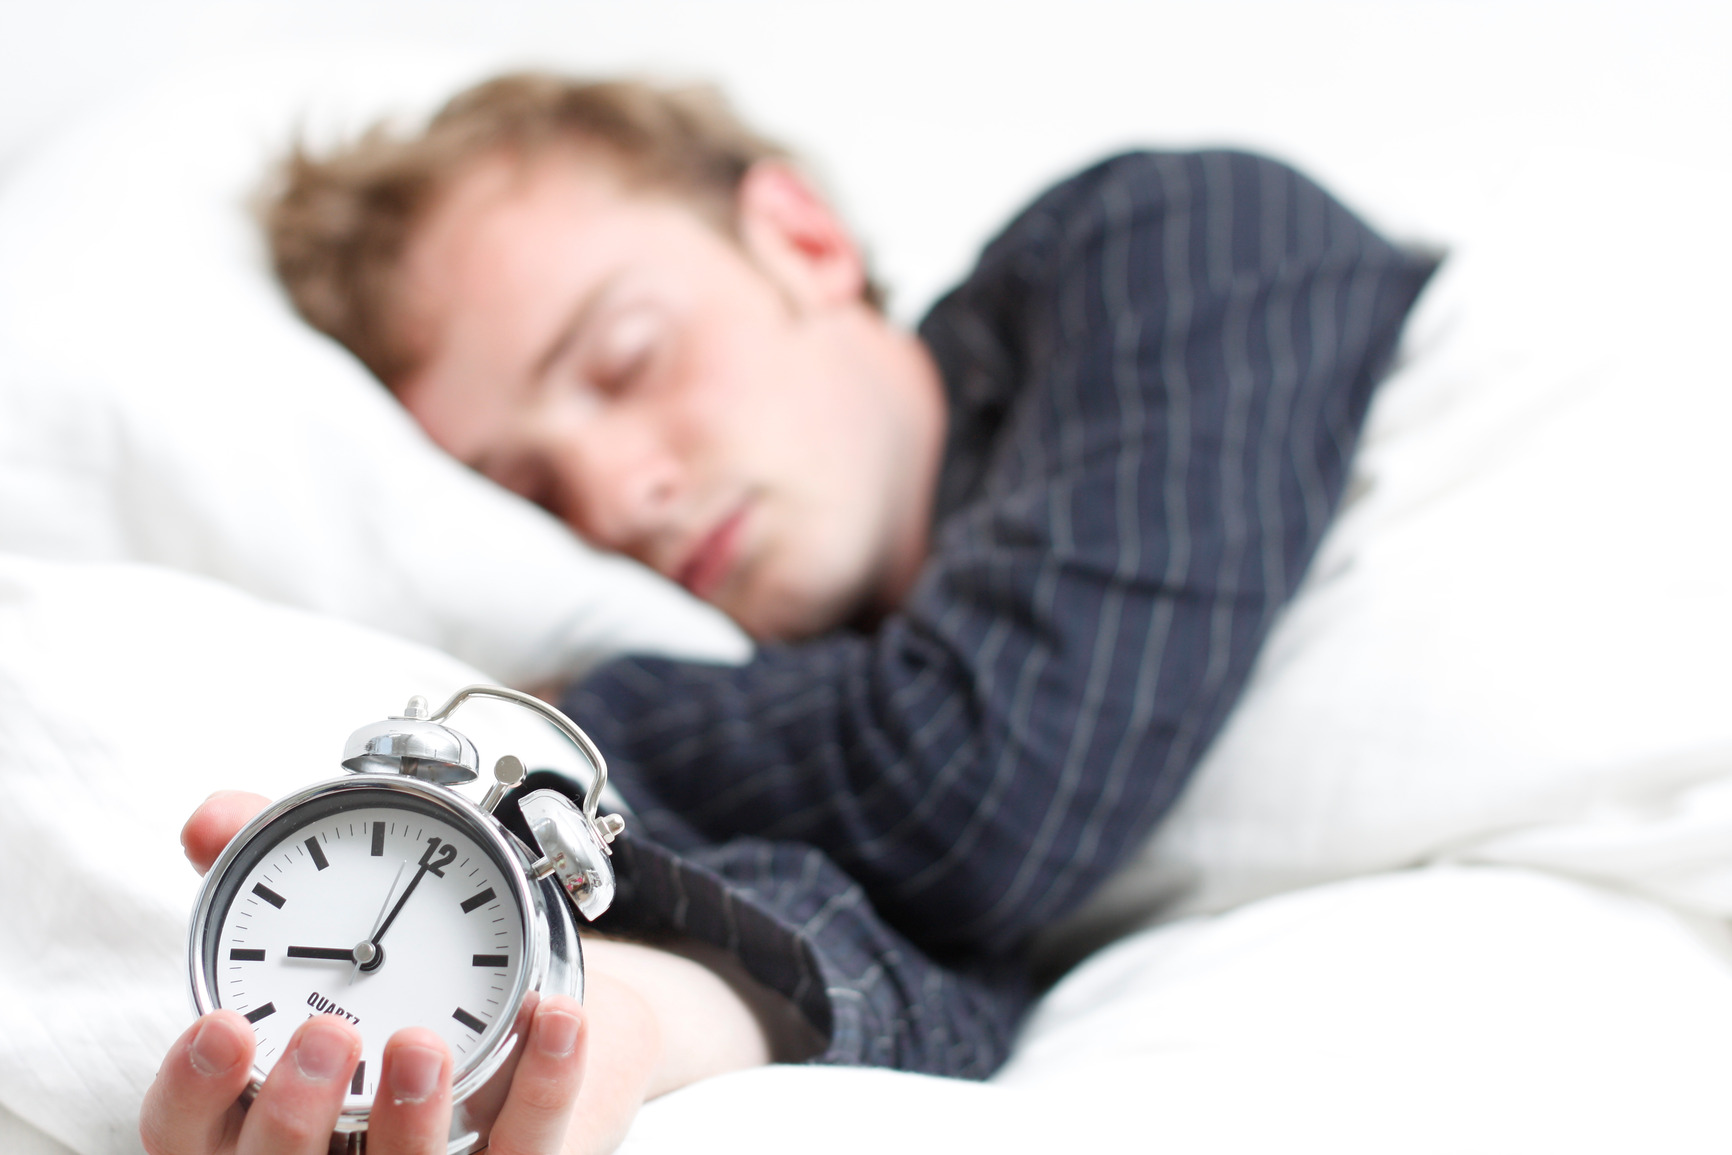
\includegraphics[width = 3cm]{ProgramsImages/Valuable-Sleep.jpg}}
	\end{tabular}
	\vspace{-5ex}
	\[L(f)  = \frac 1N \sum_{j=1}^N f(j), \qquad \cov(f,g) = \frac 1N \sum_{i=1}^N [f(j) - L(f)][g(j) - L(g)]\]
	\vspace{-1ex}	
	\centerline{\redroundmathbox{\mu - \hmu  = \begin{cases} 
				 \frac{- \cov\bigl(f, \bbone_{\{\vx_i\}_{i=1}^n}\bigr) }{\std_{\hnu} \bigl( \cov\bigl(f, \bbone_{\{\vx_i\}_{i=1}^n}\bigr)\bigr)} \, \sqrt{\frac{1-n/N}{\alert{n}(1-1/N)}} \, \std(f)  & \text{simple random}\\
			\hspace{1.1em} -\corr\bigl(f, \bbone_{\{\vx_i\}_{i=1}^n}\bigr) \hspace{1.9em}
			 \sqrt{\frac{1-n/N}{\alert{n/N}}} \hspace{0.8em}
			\std(f) & \text{web}
	\end{cases}}}
	\vspace{-3.5ex}
	\begin{itemize}
		
		\item The error of a web survey with $n_{\text{web}}$ samples is equivalent to the error of survey with   $n_{\text{SRS}} \approx \frac{n_{\text{web}}/N}{\corr^2\bigl(f, \bbone_{\{\vx_i\}_{i=1}^n}\bigr)(1-n_{\text{web}}/N)}$ simple random samples 
		
		\item E.g., $n_{\text{web}} = 125$ million distinct samples from a population of $N = 250$ million with a correlation of $0.05$ is about as valuable as $n_{\text{SRS}} = 400$ simple random samples
		
		
	\end{itemize}
\end{frame}

\begin{frame}
	\frametitle{Big Data Conclusions}
	\vspace{-6ex}
	\begin{tabular}{m{8.5cm}m{3cm}}
					\hspace{-1cm}\parbox{9.2cm}{\begin{quotation}
						\noindent With enough data, the numbers speak for themselves. \\
						\phantom{a}\hfill \href{http://www.wired.com/2008/06/pb-theory/}{\textup{Chris Anderson,} The End of Theory \\
						\phantom{a} \hfill	\textup{Wired Magazine, 2008}} \\
						\noindent \alert{``Enough'' may mean much more than you think. }
					\end{quotation}}
					&
		\hspace{-0.5cm}\href{http://www.preapps.com/blog/wp-content/uploads/2015/09/Valuable-Sleep.jpg}{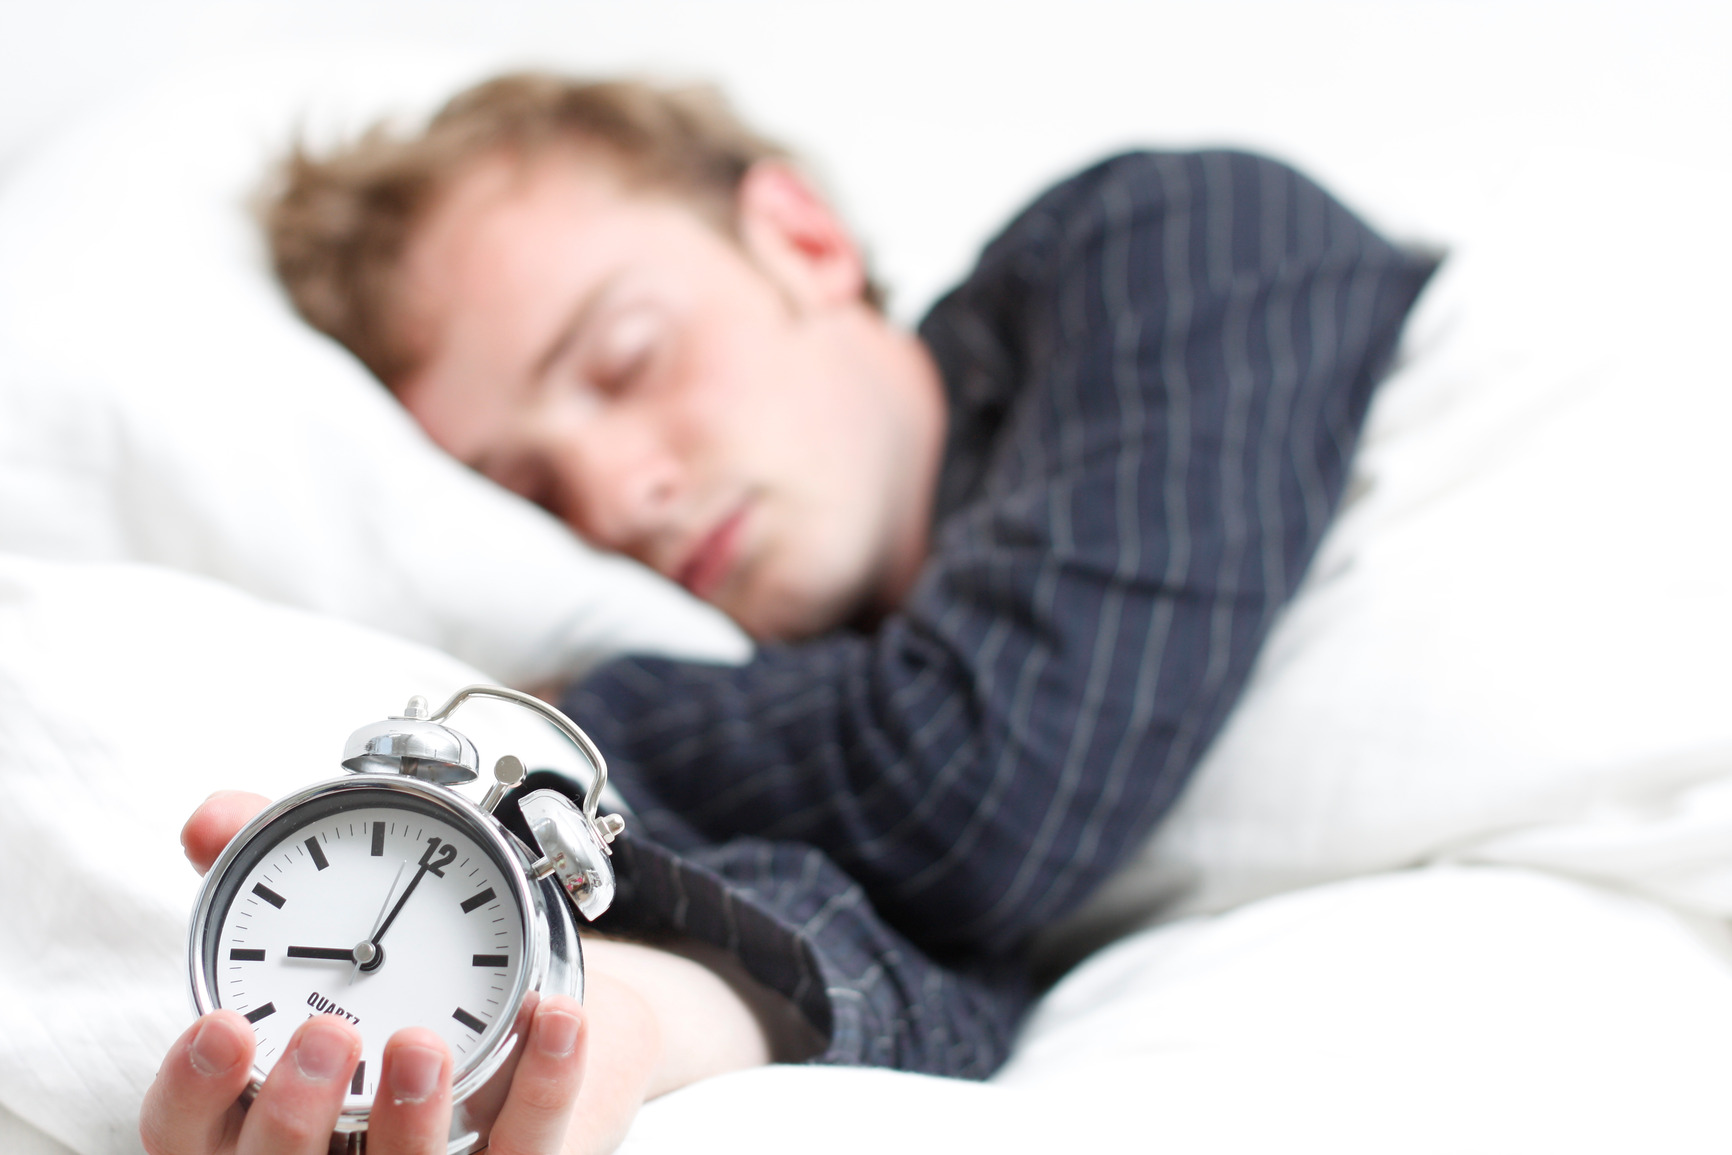
\includegraphics[width = 3cm]{ProgramsImages/Valuable-Sleep.jpg}}
	\end{tabular}
	\vspace{-2ex}	
	\centerline{\redroundmathbox{\mu - \hmu  = \begin{cases} 
				\frac{- \cov\bigl(f, \bbone_{\{\vx_i\}_{i=1}^n}\bigr) }{\std_{\hnu} \bigl( \cov\bigl(f, \bbone_{\{\vx_i\}_{i=1}^n}\bigr)\bigr)} \, \sqrt{\frac{1-n/N}{\alert{n}(1-1/N)}} \, \std(f)  & \text{simple random}\\
				\hspace{1.1em} -\corr\bigl(f, \bbone_{\{\vx_i\}_{i=1}^n}\bigr) \hspace{1.9em}
				\sqrt{\frac{1-n/N}{\alert{n/N}}} \hspace{0.8em}
				\std(f) & \text{web}
			\end{cases}}}
			\vspace{-1ex}
			\begin{itemize}
				
				\item The error of a web survey with $n_{\textrm{web}}$ samples is equivalent to the error of survey with   $n_{\textrm{SRS}} \approx \frac{n_{\text{web}}/N}{\corr^2\bigl(f, \bbone_{\{\vx_i\}_{i=1}^n}\bigr)(1-n_{\text{web}}/N)}$ simple random samples  		
				
				\item E.g., $n_{\text{web}} = 125$ million distinct samples from a population of $N = 250$ million with a correlation of $0.05$ is about as valuable as $n_{\text{SRS}} = 400$ simple random samples
								
			\end{itemize}
			
		\end{frame}


\begin{frame} \frametitle{Multivariate Normal Probability}
	\vspace{-8ex}
	\begin{tabular}{m{8.5cm}m{3cm}}
		\begin{equation*}
		\mu = \int_{[\va,\vb]} \frac{\exp\bigl(- \frac 12 \vt^T \mSigma^{-1} \vt \bigr)}{\sqrt{(2 \pi)^d \det(\mSigma)}} \, \dif \vt \
		\overset{\text{\smallocite{Gen93}}}{=} \ \int_{[0,1]^{d-1}} f(\vx) \, \dif \vx 
		\end{equation*}
		& \href{http://www.mathworks.com/matlabcentral/answers/uploaded_files/26298/Plotting\%20a\%203d\%20gaussian\%20function\%20using\%20surf\%20-\%202015\%2002\%2027.png}{\includegraphics[width = 3cm]{ProgramsImages/Plotting_gaussian.png}}
	\end{tabular}
	\vspace{-3ex}
	
	\centerline{\redroundmathbox{\mu - \hmu = 
    \begin{Bmatrix} \cos(f,\text{error rep}) & \disc^\Dt(\nu - \hnu) \\
				\algn^\Rn(f,\nu - \hnu) &  \disc^\Rn(\nu - \hnu) \end{Bmatrix} \Var^\Dt(f) }  }
	
	\vspace{-2ex}
	\begin{tabular}{m{4.5cm}m{7cm}}
		\vspace{-2ex}
		For scrambled Sobol' points
		
		\vspace{-3.5ex}
		\[
		\begin{aligned}
		\disc^\Dt(\nu - \hnu) & = \Order(n^{-1 + \epsilon})\\
		\disc^\Rn(\nu - \hnu) & = \Order(n^{\alert{-3/2} + \epsilon})
		\end{aligned}\]
		\vspace{-2.5ex}
		
		\smallcites{Owe97, HicYue00, HeiHicYue02a}
		
		\vspace{1.5ex}
		
		\noindent
		$\text{\parbox{4.5cm}{\raggedleft
				\hfill For some typical choice of \newline 
				\phantom{a}\hfill  $\va$, $\vb$, $\mSigma$, and $d=3$ \newline 
				 $\mu \approx 0.6763$}} {\color{red}\Biggr \}}$
		
		\vspace{1.5ex}
		
		\alert{Removing bias can help. \newline You might not be unlucky. }
		&
		\includegraphics[width = 7cm]{ProgramsImages/MVNIIDUSobolSobol.eps}
	\end{tabular}
	
\end{frame}

\begin{frame}
	\frametitle{Bayesian Trio Identity}
	\vspace*{-4ex}
	Error analysis assuming a random $f$ has been pursued by \cite{Dia88a}, \cite{Rit00a}  and others.
	Suppose that $f \sim \GP (0, s^2C)$,  a Gaussian process in the sample space $\cf$ with zero mean and covariance kernel $C:\cx \times \cx \to \reals$.  Let $S : \cf \to \reals$ be linear with
	$ \var_{f}\bigl(S(f)\bigr)= s^2$, $S^{\cdot}S^{\cdot\cdot}C(\cdot,\cdot\cdot) =  1$.
	Then 
	\vspace{-1ex}
	\begin{align*}
	%\mu - \hmu & \big \vert \{f(\vx_i )= y_i\}_{i=1}^n \sim \cn \bigl( \vy^T (\mC^{-1}\vc - \vw), s^2(c_0 - \vc ^T \mC^{-1} \vc) \bigr) \\
	c_0 & = \int_{\cx^2} C(\vx,\vt) \, \nu(\dif \vx) \nu(\dif \vt), \qquad \vc = \biggl( \int_{\cx} C(\vx_i,\vt) \,\nu(\dif \vt) \biggr)_{i=1}^n \\
	\mC & = \bigl( C(\vx_i,\vx_j) \bigr)_{i,j=1}^n, \qquad \vw = \bigl(w_i \bigr)_{i=1}^n,  \quad \vone^T \vw \text{ may be } \ne 1\\
	\redroundmathbox{\mu - \hmu} 
	& =  \redroundmathbox{\displaystyle%
		\underbrace{\frac{ \int_{\cx} f(\vx) \, (\nu - \hnu)(\dif\vx)}{s \sqrt{c_0 - 2 \vc^T \vw + \vw^T \mC \vw}}}_{\textstyle \algn^\Ba(f,\nu - \hnu)} \, 
		\underbrace{\sqrt{c_0 - 2 \vc^T \vw + \vw^T \mC \vw}}_{\textstyle\disc^\Ba(\nu - \hnu)} \, \underbrace{s}_{\textstyle\Var^\Ba(f)}}\\
	\algn^\Ba(f,\nu - \hnu) &\sim \cn ( 0, 1 ) \\
	\algn^\Ba(f,\nu - \hnu) & \big \vert \{f(\vx_i )= y_i\}_{i=1}^n \\
	& \sim \cn \biggl( \frac{\vy^T (\mC^{-1}\vc - \vw)}{s\sqrt{c_0 - 2 \vc^T \vw + \vw^T \mC \vw}}, \frac{c_0 - \vc ^T \mC^{-1} \vc}{c_0 - 2 \vc^T \vw + \vw^T \mC \vw} \biggr) \\
	& \sim \cn (0,1) \quad \text{if } \vw = \mC^{-1}\vc 
	\end{align*}	
\end{frame}

\begin{frame}
	\frametitle{Bayesian Trio Identity}
	\vspace*{-7ex}
	\begin{align*}
	c_0 & = \int_{\cx^2} C(\vx,\vt) \, \nu(\dif \vx) \nu(\dif \vt), \qquad \vc = \biggl( \int_{\cx} C(\vx_i,\vt) \,\nu(\dif \vt) \biggr)_{i=1}^n \\
	\mC & = \bigl( C(\vx_i,\vx_j) \bigr)_{i,j=1}^n, \qquad \vw = \bigl(w_i \bigr)_{i=1}^n,  \quad \vone^T \vw \text{ may be } \ne 1\\
	\redroundmathbox{\mu - \hmu} 
	& =  \redroundmathbox{\displaystyle%
		\underbrace{\algn^\Ba(f,\nu - \hnu)}_{\textstyle \sim \cn ( 0, 1 )} \, 
		\underbrace{\sqrt{c_0 - 2 \vc^T \vw + \vw^T \mC \vw}}_{\textstyle\disc^\Ba(\nu - \hnu)} \, \underbrace{s}_{\textstyle\Var^\Ba(f)}}
	\end{align*}
		\vspace*{-4ex}
	\begin{itemize}
		\item Bayesian analysis opens the possibility to confidence intervals for $\mu$ even if $\hnu$ is deterministic
		\item But how do you estimate $s$ plus any parameters lurking in $C$?
		\item $\disc^\Ba(\nu - \hnu) = \disc^\Dt(\nu - \hnu)$ for RKHS with $K$ replaced by $C$
		\item $\vw  = \mC^{-1}\vc$ minimizes the discrepancy in both the Bayesian and deterministic RKHS cases, but 
		\begin{itemize}
			\item generally requires $\Order(n^3)$ operations, and
			\item $\hmu$ might not integrate constants exactly
		\end{itemize}
		\item May also consider optimizing placement of data sites, $\{\vx_i\}_{i=1}^n$, but this is more difficult \cite{}
	\end{itemize}
	
\end{frame}

\begin{frame} \frametitle{Multivariate Normal Probability}
	\vspace{-8ex}
	\begin{tabular}{m{8.5cm}m{3cm}}
		\begin{equation*}
		\mu = \int_{[\va,\vb]} \frac{\exp\bigl(- \frac 12 \vt^T \mSigma^{-1} \vt \bigr)}{\sqrt{(2 \pi)^d \det(\mSigma)}} \, \dif \vt \
		\overset{\text{\smallocite{Gen93}}}{=} \ \int_{[0,1]^{d-1}} f(\vx) \, \dif \vx 
		\end{equation*}
		& \href{http://www.mathworks.com/matlabcentral/answers/uploaded_files/26298/Plotting\%20a\%203d\%20gaussian\%20function\%20using\%20surf\%20-\%202015\%2002\%2027.png}{\includegraphics[width = 3cm]{ProgramsImages/Plotting_gaussian.png}}
	\end{tabular}
	\vspace{-3ex}
	
	\centerline{\redroundmathbox{\mu - \hmu = 
			\begin{Bmatrix} \cos(f,\text{error rep}) & \disc^\Dt(\nu - \hnu) \Var^\Dt(f) \\
				\algn^\Rn(f,\nu - \hnu) &  \disc^\Rn(\nu - \hnu)  \Var^\Dt(f)  \\
				\algn^\Ba(f,\nu - \hnu) &  \disc^\Ba(\nu - \hnu)  \Var^\Ba(f) \end{Bmatrix}}}
	
	\vspace{-2ex}
	\begin{tabular}{m{4.5cm}m{7cm}}
		\vspace{-2ex}
		Improved convergence for smoother integrands using an \alert{optimally} (unequally) weighted sample average with scrambled Sobol' data sites 
		
		\vspace{1.5ex}
		
		\noindent
		$\text{\parbox{4.5cm}{\raggedleft
				\hfill For some typical choice of \newline 
				\phantom{a}\hfill  $\va$, $\vb$, $\mSigma$, and $d=3$ \newline 
				$\mu \approx 0.6763$}} {\color{red}\Biggr \}}$
		
		\vspace{1.5ex}
		
		\alert{Computing the weights is time consuming, but could be done offline }
		&
		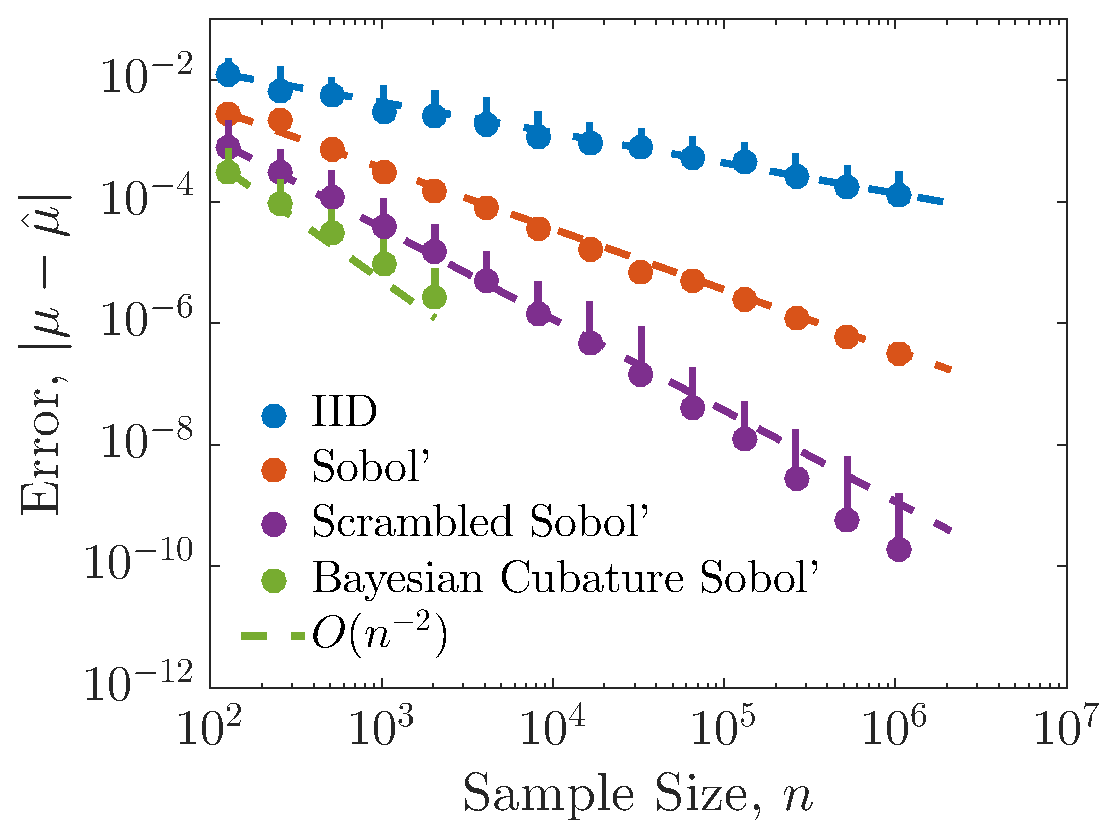
\includegraphics[width = 7cm]{ProgramsImages/MVNIIDUSobolSobolWtSobol.eps}
	\end{tabular}
	
\end{frame}

\begin{frame}
	\frametitle{Randomized Bayesian Trio Identity}
		\vspace*{-4ex}
		Assume that $f \sim \GP (0, s^2C)$ and $\hnu$ is random (independent of $f$).  Then 
		\vspace{-1ex}
		\begin{align*}
		c_0 & = \int_{\cx^2} C(\vx,\vt) \, \nu(\dif \vx) \nu(\dif \vt), \qquad \vc = \biggl( \int_{\cx} C(\vx_i,\vt) \,\nu(\dif \vt) \biggr)_{i=1}^n \\
		\mC &= \bigl( C(\vx_i,\vx_j) \bigr)_{i,j=1}^n\\
		\redroundmathbox{\mu - \hmu} 
		& =  \redroundmathbox{\displaystyle%
			\underbrace{\frac{ \int_{\cx} f(\vx) \, (\nu - \hnu)(\dif\vx)}{s \sqrt{\Ex_{\hnu}\bigl(c_0 - 2 \vc^T \vw + \vw^T \mC \vw\bigr)}}}_{\textstyle \algn^{\Ba\Rn}(f,\nu - \hnu) \sim \cn ( 0, 1 )} \, 
			\underbrace{\sqrt{\Ex_{\hnu}\bigl(c_0 - 2 \vc^T \vw + \vw^T \mC \vw\bigr)}}_{\textstyle\disc^{\Ba\Rn}(\nu - \hnu)} \, \underbrace{s}_{\textstyle\Var^\Ba(f)}}
		\end{align*}

\end{frame}

\begin{frame}
	\frametitle{Randomized Bayesian Trio Identity}
	\vspace*{-4ex}
	$f \sim \GP (0, s^2C)$ and $\hnu$ is random (independent of $f$):
	\vspace{-1ex}
	\begin{align*}
	\redroundmathbox{\mu - \hmu} 
	& =  \redroundmathbox{\displaystyle%
		\underbrace{\frac{ \int_{\cx} f(\vx) \, (\nu - \hnu)(\dif\vx)}{s \sqrt{\Ex_{\hnu}\bigl(c_0 - 2 \vc^T \vw + \vw^T \mC \vw\bigr)}}}_{\textstyle \algn^{\Ba\Rn}(f,\nu - \hnu) \sim \cn ( 0, 1 )} \, 
		\underbrace{\sqrt{\Ex_{\hnu}\bigl(c_0 - 2 \vc^T \vw + \vw^T \mC \vw\bigr)}}_{\textstyle\disc^{\Ba\Rn}(\nu - \hnu)} \, \underbrace{s}_{\textstyle\Var^\Ba(f)}}
	\end{align*}
	For $\vw  = \vone/n$, and unbiased estimation:
	\[
	\disc^{\Ba\Rn}(\nu - \hnu) = \sqrt{\frac {\vone^T \tmC \vone}{n^2} - c_0 }, \qquad \tmC  = \Bigl(\Ex_{\hnu} C(\vx_i,\vx_j) \Bigr)_{i,j=1}^n
	\]	
	For some $\{\vx_i\}_{i=1}^n$, such as scrambled nets and shifted integration lattices
	\[
	\disc^{\Ba\Rn}(\nu - \hnu) = \sqrt{ \frac {\vone^T\tvC_1}{n} - c_0 }, \qquad \tmC  = (\tvC_1, \ldots, \tvC_n)
	\]	
	which requires only $\Order(n)$ operations to evaluate \cite{??}
	
\end{frame}



\section{Tractability}

\begin{frame}
	content...
\end{frame}


\section{Rewriting the Problem}

\begin{frame}
	content...
\end{frame}


\section{When to Stop}
\begin{frame}
	content...
\end{frame}


\begin{frame}[allowframebreaks]\frametitle{References}
	\bibliography{FJH23,FJHown23}
\end{frame}

\end{document}



